%!TEX program = xelatex
%!TEX root = ../all_beamer.tex


% SVM Beamer Presentation
% Based on notes by Giorgio Gambosi, University of Rome "Tor Vergata"
% Style inspired by the SLT Beamer template

%% !TEX root = all_beamer.tex
% ==============================================================================
% HEADER LATEX PER PRESENTAZIONI BEAMER
% Corso di Machine Learning - Giorgio Gambosi
% Università di Roma "Tor Vergata"
% ==============================================================================

% ------------------------------------------------------------------------------
% CLASSE DOCUMENTO E METADATI
% ------------------------------------------------------------------------------
\documentclass[aspectratio=169, 10pt]{beamer}

\subtitle{Course of Machine Learning}
\author{Giorgio Gambosi}
\institute[Tor Vergata]{Master's Degree in Computer Science\\University of Rome ``Tor Vergata''}
\date{A.Y. 2025--2026}

% ------------------------------------------------------------------------------
% PACCHETTI MATEMATICI
% ------------------------------------------------------------------------------
\usepackage{amsmath, amssymb, amsfonts, mathtools, amsthm}
\usepackage{bm}              % Simboli matematici in grassetto
\usepackage{upgreek}         % Lettere greche dritte
\usepackage{derivative}      % Gestione semplificata delle derivate

% ------------------------------------------------------------------------------
% PACCHETTI GRAFICI E VISUALIZZAZIONE
% ------------------------------------------------------------------------------
\usepackage{graphicx}        % Inclusione immagini
\usepackage{xcolor}          % Gestione colori
\usepackage{xkcdcolors}      % Colori aggiuntivi stile xkcd
\usepackage{microtype}       % Miglioramenti tipografici

% ------------------------------------------------------------------------------
% PACCHETTI PER TABELLE
% ------------------------------------------------------------------------------
\usepackage{booktabs}        % Tabelle professionali
\usepackage{array}           % Estensioni per tabelle
\usepackage{multirow}        % Celle multi-riga
\usepackage{multicol}        % Layout multi-colonna

% ------------------------------------------------------------------------------
% TIKZ E PGFPLOTS
% ------------------------------------------------------------------------------
\usepackage{tikz}
\usepackage{tikz-network}
\usepackage[customcolors]{hf-tikz}
\usepackage{pgfplots}
\pgfplotsset{compat=1.18}
\usepgfplotslibrary{fillbetween}

% Librerie TikZ
\usetikzlibrary{arrows, arrows.meta, decorations.pathmorphing, decorations.pathreplacing}
\usetikzlibrary{decorations.markings, snakes, positioning, backgrounds, fit, shadows}
\usetikzlibrary{automata, patterns, calc, intersections, through, shapes}
\usetikzlibrary{shapes.geometric, shapes.arrows, scopes, chains, matrix}

% ------------------------------------------------------------------------------
% ALTRI PACCHETTI
% ------------------------------------------------------------------------------
\usepackage[skins]{tcolorbox}  % Box colorati
\usepackage{subcaption}         % Sottocaption per figure
\usepackage{listings}           % Inclusione codice sorgente

% ------------------------------------------------------------------------------
% TEMA E STILE BEAMER
% ------------------------------------------------------------------------------
\usetheme{Madrid}
\usecolortheme{whale}
\useinnertheme{rounded}
\usefonttheme{professionalfonts}
\setbeamertemplate{navigation symbols}{}  % Rimuove simboli di navigazione

% ------------------------------------------------------------------------------
% DEFINIZIONE COLORI PERSONALIZZATI
% ------------------------------------------------------------------------------
% Colori principali del tema
\definecolor{MainBlue}{RGB}{31,56,100}      % Blu principale (header, titoli)
\definecolor{AccentBlue}{RGB}{70,130,180}   % Blu accento (blocchi)
\definecolor{AlertRed}{RGB}{160,30,30}      % Rosso per alert
\definecolor{ExGreen}{RGB}{30,120,60}       % Verde per esempi
\definecolor{BlockBg}{RGB}{220,232,246}     % Sfondo blocchi
\definecolor{torgray}{RGB}{220,225,235}     % Grigio Tor Vergata

% Colori alternativi (Tor Vergata style)
\definecolor{TvDark}{RGB}{30,50,80}         % Blu scuro header
\definecolor{TvMid}{RGB}{70,100,140}        % Blu medio blocchi
\definecolor{TvLight}{RGB}{210,220,235}     % Blu chiaro sfondi
\definecolor{TvAlert}{RGB}{160,30,30}       % Rosso alert
\definecolor{TvGreen}{RGB}{20,100,50}       % Verde esempi

% Colori supplementari
\definecolor{torred}{RGB}{153,0,0}
\definecolor{torcyan}{RGB}{0,112,192}
\definecolor{cerise}{HTML}{DA3A62}
\definecolor{teal}{HTML}{029386}
\definecolor{slateblue}{HTML}{5B5EA6}
\definecolor{orange}{HTML}{F97306}

% Colori per nodi TikZ
\definecolor{nodeblue}{RGB}{101,140,196}    % xkcd Faded Blue

% ------------------------------------------------------------------------------
% CONFIGURAZIONE COLORI BEAMER
% ------------------------------------------------------------------------------
\setbeamercolor{frametitle}{bg=MainBlue, fg=white}
\setbeamercolor{title}{bg=MainBlue, fg=white}
\setbeamercolor{structure}{fg=MainBlue}

% Blocchi standard
\setbeamercolor{block title}{bg=AccentBlue, fg=white}
\setbeamercolor{block body}{bg=BlockBg}

% Blocchi alert
\setbeamercolor{block title alerted}{bg=AlertRed, fg=white}
\setbeamercolor{block body alerted}{bg=red!8}

% Blocchi esempio
\setbeamercolor{block title example}{bg=ExGreen, fg=white}
\setbeamercolor{block body example}{bg=green!7}

% ------------------------------------------------------------------------------
% CONFIGURAZIONE FONT BEAMER
% ------------------------------------------------------------------------------
\setbeamerfont{frametitle}{size=\normalsize,series=\bfseries}
\setbeamerfont{block title}{size=\small,series=\bfseries}

% ------------------------------------------------------------------------------
% STILI TIKZ PERSONALIZZATI
% ------------------------------------------------------------------------------
\tikzset{
  >=latex,  % Frecce stile LaTeX di default
  % Nodi per reti neurali
  node/.style={thick,circle,draw=myblue,minimum size=22,inner sep=0.5,outer sep=0.6},
  node in/.style={node,green!20!black,draw=mygreen!30!black,fill=mygreen!25},
  node hidden/.style={node,blue!20!black,draw=myblue!30!black,fill=myblue!20},
  node convol/.style={node,orange!20!black,draw=myorange!30!black,fill=myorange!20},
  node out/.style={node,red!20!black,draw=myred!30!black,fill=myred!20},
  % Connessioni
  connect/.style={thick,mydarkblue},
  connect arrow/.style={-{Latex[length=4,width=3.5]},thick,mydarkblue,shorten <=0.5,shorten >=1},
  % Stili numerati per facile mappatura
  node 1/.style={node in},
  node 2/.style={node hidden},
  node 3/.style={node out}
}

% ------------------------------------------------------------------------------
% AMBIENTI TEOREMI
% ------------------------------------------------------------------------------
\setbeamertemplate{theorems}[numbered]
\newtheorem{mytheorem}{Theorem}
\newtheorem{mydefinition}{Definition}

% ------------------------------------------------------------------------------
% CONFIGURAZIONE LISTINGS (CODICE)
% ------------------------------------------------------------------------------
\lstset{
  language=Python,
  basicstyle=\ttfamily\tiny,
  keywordstyle=\color{MainBlue}\bfseries,
  commentstyle=\color{gray},
  frame=single,
  breaklines=true,
}

% ==============================================================================
% MACRO MATEMATICHE PERSONALIZZATE
% ==============================================================================

% ------------------------------------------------------------------------------
% SPAZI CALLIGRAFICI (Calligraphic spaces)
% ------------------------------------------------------------------------------
\providecommand{\calX}{\mathcal{X}}         % Spazio input
\providecommand{\calY}{\mathcal{Y}}         % Spazio output
\providecommand{\calH}{\mathcal{H}}         % Spazio ipotesi
\providecommand{\calT}{\mathcal{T}}         % Training set
\providecommand{\calA}{\mathcal{A}}         % Algoritmo
\providecommand{\calR}{\mathcal{R}}         % Rischio
\providecommand{\calF}{\mathcal{F}}         % Famiglia di funzioni
\providecommand{\calL}{\mathcal{L}}         % Loss function

% Alias per compatibilità
\providecommand{\Rr}{\mathcal{R}}
\providecommand{\Tr}{\mathcal{T}}
\providecommand{\Hr}{\mathcal{H}}

% ------------------------------------------------------------------------------
% RISCHIO E PROBABILITÀ
% ------------------------------------------------------------------------------
\providecommand{\barR}{\overline{\mathcal{R}}}  % Rischio empirico
\providecommand{\EmpR}{\overline{\mathcal{R}}}  % Rischio empirico (alias)
\providecommand{\Rbar}{\overline{\mathcal{R}}}  % Rischio empirico (alias)
\providecommand{\pM}{p_M}                       % Probabilità modello
\providecommand{\pC}{p_C}                       % Probabilità corretta
\providecommand{\Prob}[2]{\mathbb{P}_{#1}\!\left[#2\right]}  % Probabilità

% ------------------------------------------------------------------------------
% FUNZIONI INDICATRICI
% ------------------------------------------------------------------------------
\providecommand{\indicator}[1]{\mathbf{1}\!\left[#1\right]}  % Funzione indicatrice
\providecommand{\ind}[1]{\mathbf{1}[#1]}                      % Versione breve

% ------------------------------------------------------------------------------
% OPERATORI MATEMATICI
% ------------------------------------------------------------------------------
\providecommand{\argmax}{\operatorname*{arg\,max}}  % Argomento del massimo
\providecommand{\argmin}{\operatorname*{arg\,min}}  % Argomento del minimo
\providecommand{\vcd}[1]{\operatorname{VCdim}(#1)} % VC dimension
\providecommand{\defeq}{\stackrel{\text{def}}{=}}  % Definito come

% ------------------------------------------------------------------------------
% VETTORI E MATRICI (Bold Math)
% ------------------------------------------------------------------------------
% Vettori minuscoli
\providecommand{\bx}{\mathbf{x}}            % Vettore x
\providecommand{\bz}{\mathbf{z}}            % Vettore z
\providecommand{\bw}{\mathbf{w}}            % Vettore peso
\providecommand{\btt}{\mathbf{t}}           % Vettore target
\providecommand{\wvec}{\mathbf{w}}          % Vettore peso (alias)
\providecommand{\bth}{\boldsymbol{\theta}}  % Parametro theta

% Matrici maiuscole
\providecommand{\bX}{\mathbf{X}}            % Matrice dati
\providecommand{\bZ}{\mathbf{Z}}            % Matrice Z
\providecommand{\Xmat}{\mathbf{X}}          % Matrice dati (alias)
\providecommand{\Hmat}{\mathbf{H}}          % Matrice H
\providecommand{\Smat}{\mathbf{S}}          % Matrice scatter generica
\providecommand{\bS}{\mathbf{S}}            % Matrice scatter
\providecommand{\Ii}{\mathbf{I}}            % Matrice identità
\providecommand{\bZero}{\mathbf{0}}         % Vettore zero
\providecommand{\bPsi}{\boldsymbol{\Psi}}   % Matrice Psi

% Medie (overline)
\providecommand{\ox}{\overline{\mathbf{x}}} % Media vettore x
\providecommand{\ow}{\overline{\mathbf{w}}} % Media vettore w
\providecommand{\oX}{\overline{\mathbf{X}}} % Media matrice X

% Matrici scatter specifiche (analisi discriminante)
\providecommand{\SW}{\mathbf{S}_W}          % Within-class scatter
\providecommand{\SB}{\mathbf{S}_B}          % Between-class scatter
\providecommand{\ST}{\mathbf{S}_T}          % Total scatter
\providecommand{\GX}{G_{\mathbf{X}}}        % Matrice Gram

% ------------------------------------------------------------------------------
% COMANDI DI FORMATTAZIONE TESTO
% ------------------------------------------------------------------------------
\providecommand{\term}[1]{\textbf{\color{accent}#1}}        % Termine importante
\providecommand{\halert}[1]{{\color{AlertRed}\textbf{#1}}}  % Alert rosso
\providecommand{\mlalert}[1]{{\color{AccentBlue}\textbf{#1}}}  % Alert blu
\providecommand{\mlemph}[1]{{\color{MainBlue}\textit{#1}}}  % Enfasi blu

% ==============================================================================
% FINE HEADER
% ==============================================================================

\newcommand{\blankpage}{
\clearpage
\thispagestyle{empty}
\null
\clearpage
}

% ---------- Packages ----------
%\usepackage{amsmath, amssymb, mathtools, amsthm}
%\usepackage{booktabs}
%\usepackage{tikz}
%\usetikzlibrary{arrows.meta, positioning, shapes.geometric, fit}
%\usepackage{xcolor}
%\usepackage{microtype}
%\usepackage{graphicx}

% ---------- Theorem styles ----------
%\setbeamertemplate{theorems}[numbered]
%\newtheorem{mytheorem}{Theorem}
%\newtheorem{mydefinition}{Definition}
%
%% ---------- Macros ----------
%
%\newcommand{\calX}{\mathcal{X}}
%\newcommand{\calY}{\mathcal{Y}}
%\newcommand{\calH}{\mathcal{H}}
%\newcommand{\calT}{\mathcal{T}}
%\newcommand{\calA}{\mathcal{A}}
%\newcommand{\calR}{\mathcal{R}}
%\newcommand{\calF}{\mathcal{F}}
%\newcommand{\barR}{\overline{\mathcal{R}}}
%\newcommand{\pM}{p_M}
%\newcommand{\pC}{p_C}
%\newcommand{\indicator}[1]{\mathbf{1}\!\left[#1\right]}
%\newcommand{\vcd}[1]{\operatorname{VCdim}(#1)}
%\newcommand{\Prob}[2]{\mathbb{P}_{#1}\!\left[#2\right]}
%% ---------- Theme ----------
%% ---------- Custom colours (matching PDF model) ----------
%\definecolor{TvDark}{RGB}{30,50,80}        % dark navy for header bar
%\definecolor{TvMid}{RGB}{70,100,140}       % medium blue for blocks
%\definecolor{TvLight}{RGB}{210,220,235}    % pale blue for backgrounds
%\definecolor{TvAlert}{RGB}{160,30,30}      % dark red for alerts / warnings
%\definecolor{TvGreen}{RGB}{20,100,50}      % green for examples

% ---------- Beamer colours ----------
%\setbeamercolor{frametitle}{bg=TvDark, fg=white}
%\setbeamercolor{framesubtitle}{fg=TvLight}
%\setbeamercolor{structure}{fg=TvMid}
%\setbeamercolor{block title}{bg=TvMid, fg=white}
%\setbeamercolor{block body}{bg=TvLight, fg=black}
%\setbeamercolor{block title alerted}{bg=TvAlert, fg=white}
%\setbeamercolor{block body alerted}{bg=TvLight!60!red!20, fg=black}
%\setbeamercolor{block title example}{bg=TvGreen, fg=white}
%\setbeamercolor{block body example}{bg=TvLight!60!green!20, fg=black}
%\setbeamercolor{footline}{fg=TvMid}
%\setbeamercolor{title}{fg=TvDark}
%\setbeamercolor{subtitle}{fg=TvMid}
%
%% ---------- Beamer fonts ----------
%\setbeamerfont{frametitle}{size=\large, series=\bfseries}
%\setbeamerfont{framesubtitle}{size=\small, series=\normalfont}
%\setbeamerfont{block title}{size=\normalsize, series=\bfseries}
%\setbeamerfont{footline}{size=\tiny}
%
%% ---------- Frame title with subsection ----------
%\setbeamertemplate{frametitle}{%
%  \vspace{0.3em}
%  \insertframetitle
%  \ifx\insertframesubtitle\empty\else
%    \\[0.1em]
%    {\usebeamerfont{framesubtitle}\usebeamercolor[fg]{framesubtitle}\insertframesubtitle}
%  \fi
%}
%
%% ---------- Footline ----------
%\setbeamertemplate{footline}{%
%  \hbox{%
%    \begin{beamercolorbox}[wd=0.33\paperwidth, ht=2.25ex, dp=1ex, leftskip=2mm]{footline}%
%      \insertshortauthor
%    \end{beamercolorbox}%
%    \begin{beamercolorbox}[wd=0.34\paperwidth, ht=2.25ex, dp=1ex, center]{footline}%
%      \insertshorttitle
%    \end{beamercolorbox}%
%    \begin{beamercolorbox}[wd=0.33\paperwidth, ht=2.25ex, dp=1ex, rightskip=2mm, right]{footline}%
%      \insertframenumber{} / \inserttotalframenumber
%    \end{beamercolorbox}%
%  }%
%}
%
%\setbeamertemplate{navigation symbols}{}
%
%% ---------- Bullets ----------
%\setbeamertemplate{itemize item}{\textcolor{TvMid}{\textbullet}}
%\setbeamertemplate{itemize subitem}{\textcolor{TvMid}{--}}

% ---------- Macros ----------
%\newcommand{\w}{\mathbf{w}}
%\newcommand{\x}{\mathbf{x}}
%\newcommand{\Vlambda}{\boldsymbol{\lambda}}
%\newcommand{\Vxi}{\boldsymbol{\xi}}


% ---------- Title info ----------
\title{Support Vector Machines}
%\subtitle{Course of Machine Learning}
%\author{Giorgio Gambosi}
%\institute{Master's Degree in Computer Science\\University of Rome ``Tor Vergata''}
%\date{A.Y.\ 2025--2026}
%
%% ==========================================================================
%\begin{document}
% ==========================================================================

\begin{frame}
  \titlepage
\end{frame}

% ---------- Outline ----------
\begin{frame}{Outline}
  \tableofcontents
\end{frame}

% ==========================================================================
\section{Introduction and Linear Classifiers}
% ==========================================================================

\begin{frame}{The Core Idea of SVMs}
  \framesubtitle{Why margin matters}
  \begin{block}{What SVMs do}
    SVMs find the \alert{optimal} separating hyperplane: one that maximises
    the \alert{margin} between the two classes.
  \end{block}
  \vspace{0.5em}
  \begin{itemize}
    \item Goal: binary classification with a linear decision boundary.
    \item Not just any separating hyperplane — the \emph{widest possible} one.
    \item Two practical challenges arise:
      \begin{itemize}
        \item Data may not be perfectly linearly separable $\;\Rightarrow\;$
              \alert{soft margins}.
        \item Linear separation may fail in original space $\;\Rightarrow\;$
              \alert{kernel trick}.
      \end{itemize}
  \end{itemize}
\end{frame}

\begin{frame}{Classification Scores}
  \framesubtitle{From numbers to labels}
  \begin{itemize}
    \item Most classifiers compute a numerical \alert{score}:
          \[
            \text{score}(\x) = \w^T\x + b.
          \]
    \item $\w$ — orientation of the boundary;\quad $b$ — its position.
    \item Final label: $\hat{y} = \mathrm{sign}(\w^T\x + b)$.
  \end{itemize}
  \vspace{0.4em}
  \begin{block}{Geometric meaning}
    \begin{itemize}
      \item Points with $\w^T\x + b = 0$: exactly on the \alert{decision boundary}.
      \item Sign of the score: which side of the boundary.
      \item Magnitude: distance from the boundary (scaled by $\|\w\|$).
    \end{itemize}
  \end{block}
\end{frame}

\begin{frame}{Decision Boundary — Geometric Illustration}
  \framesubtitle{Score as signed distance}
  \begin{columns}
    \column{0.5\textwidth}
      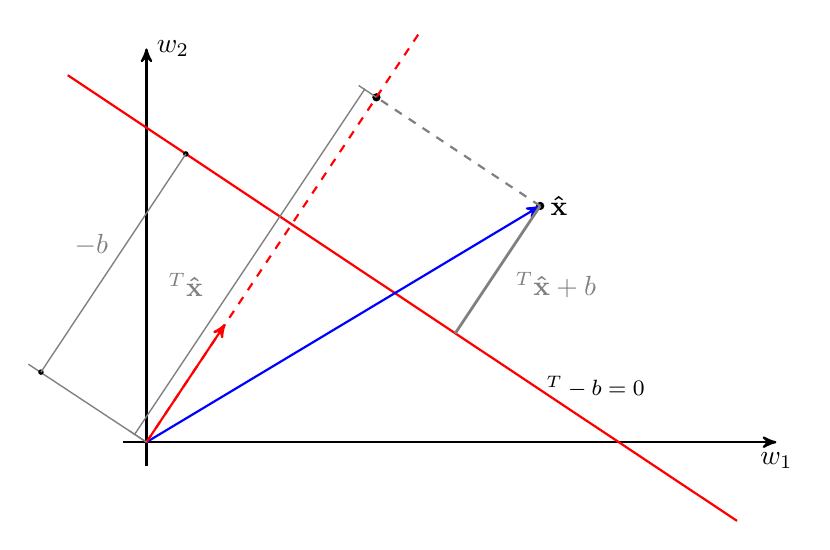
\begin{tikzpicture}[
    thick,
    >=stealth',
    dot/.style = {
      draw,
      fill = white,
      circle,
      inner sep = 0pt,
      minimum size = 4pt
    }
  ]
  \coordinate (O) at (0,0);
  \draw[->] (-0.3,0) -- (8,0) coordinate[label = {below:$w_1$}] (xmax);
  \draw[->] (0,-0.3) -- (0,5) coordinate[label = {right:$w_2$}] (ymax);
  \path[name path=x] (0.3,0.5) -- (6.7,4.7);
  \path[name path=y] plot[smooth] coordinates {(-0.3,2) (2,1.5) (4,2.8) (6,5)};
  \scope[name intersections = {of = x and y, name = i}]
    \draw[red] (-1,4.66) -- (7.5,-1) node[pos=0.7,  right] {\color{black}\footnotesize$\w^T\x-b=0$};
     \fill (5,3) circle (1.5pt);
    \node[right] at (5,3) {$\mathbf{\hat x}$};
     \draw[blue, ->] (0,0) --  (5,3);
      \fill (2.92,4.38) circle (1.5pt);
      \draw[gray,dashed](5,3)--(2.92,4.38);
    \draw[red, ->] (0,0) -- node[right] {$\w$} (1,1.5);
    \draw[red, dashed] (0,0) -- (3.5,5.25);
    
     \fill (-.15,.1) circle (.3pt);
     \fill (2.77,4.48) circle (.3pt);
     \draw[gray, line width=.5pt] (-.225,.15) -- (0,0);
     \draw[gray, line width=.5pt] (-.15,.1) -- (2.77,4.48);
     \draw[gray, line width=.5pt] (2.92,4.38) -- (2.695,4.53);
     \node[gray] at (.5,2) {$\w^T\mathbf{\hat x}$};
      \draw[gray, line width=.5pt] (-1.5,.99) -- (0,0);
       \fill (.5,3.66) circle (1pt);
       \fill (-1.34,.89) circle (1pt);
        \draw[gray, line width=.5pt] (.5,3.66) -- (-1.34,.89);
        \node[gray] at (-.7,2.5) {$-b$};
         \draw[gray, line width=1pt] (5,3) -- (3.92,1.38);
          \node[gray] at (5.2,2) {$\w^T\mathbf{\hat x}+b$};
  \endscope
\end{tikzpicture}    \column{0.45\textwidth}
      \begin{itemize}
        \item $\w^T\hat{\x} + b$: \alert{signed distance} from the hyperplane.
        \item Positive $\Rightarrow$ class $+1$ side.
        \item Negative $\Rightarrow$ class $-1$ side.
        \item Large magnitude $\Rightarrow$ high-confidence prediction.
      \end{itemize}
  \end{columns}
\end{frame}

\begin{frame}{Margin and Confidence}
  \framesubtitle{Points far from the boundary are classified more confidently}
  \begin{columns}
    \column{0.45\textwidth}
     \centerline{

\includegraphics[width=.9\linewidth]{figs/largemargin.pdf}
}
    \column{0.50\textwidth}
      \begin{itemize}
        \item Point $A$: far from the boundary $\Rightarrow$ \alert{high confidence}.
        \item Point $C$: close to the boundary $\Rightarrow$ \alert{uncertain} decision.
        \item Intuition: a classifier that pushes training points away from the boundary should \emph{generalise better}.
        \item This motivates maximising the \alert{margin}.
      \end{itemize}
  \end{columns}
\end{frame}

% ==========================================================================
\section{Margin: Formal Definition}
% ==========================================================================

\begin{frame}{Functional Margin}
  \framesubtitle{A signed confidence measure}
  \begin{itemize}
    \item Labels: $t_i \in \{-1, +1\}$; classifier: $h(\x) = \mathrm{sign}(\w^T\x+b)$.
    \item \alert{Functional margin} of example $(\x_i, t_i)$:
          \[
            \bar{\gamma}_i = t_i(\w^T\x_i + b).
          \]
    \item Positive iff the point is \alert{correctly classified}.
    \item Larger magnitude $\Rightarrow$ greater confidence.
    \item Functional margin of the training set:
          \[
            \bar{\gamma} = \min_i \bar{\gamma}_i.
          \]
  \end{itemize}
  \begin{alertblock}{Key limitation}
    $\bar{\gamma}$ is \alert{not scale-invariant}: multiplying $(\w,b)$ by $\alpha > 0$ multiplies
    $\bar{\gamma}_i$ by $\alpha$, without changing the classifier.
  \end{alertblock}
\end{frame}

\begin{frame}{Geometric Margin}
  \framesubtitle{True Euclidean distance to the hyperplane}
  \begin{block}{Definition}
    \[
      \gamma_i = \frac{\bar{\gamma}_i}{\|\w\|} = t_i\!\left(\frac{\w^T}{\|\w\|}\x_i + \frac{b}{\|\w\|}\right).
    \]
  \end{block}
  \begin{itemize}
    \item $\gamma_i$ is the \alert{signed Euclidean distance} from $\x_i$ to the hyperplane.
    \item \alert{Scale-invariant}: unchanged by rescaling $(\w,b)$.
    \item Margin of the training set: $\gamma = \min_i \gamma_i$.
    \item $\gamma$ = half the width of the largest empty slab around the boundary.
  \end{itemize}
\end{frame}

\begin{frame}{Geometric Margin — Illustration}
  \framesubtitle{Support vectors and the margin slab}
  \begin{columns}
    \column{0.48\textwidth}
      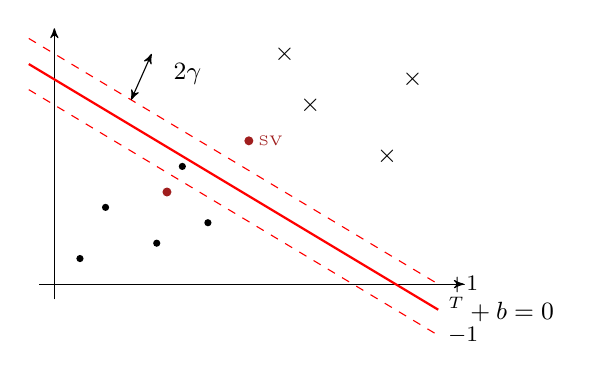
\begin{tikzpicture}[scale=0.65, >=stealth']
        \draw[->] (-.3,0) -- (8,0);
        \draw[->] (0,-.3) -- (0,5);
        \draw[red, thick] (-0.5,4.3) -- (7.5,-0.5) node[right, black]{\small $\w^T\x+b=0$};
        \draw[red, dashed] (-0.5,4.8) -- (7.5,0) node[right, black]{\footnotesize $+1$};
        \draw[red, dashed] (-0.5,3.8) -- (7.5,-1) node[right, black]{\footnotesize $-1$};
        \draw[<->] (1.5,3.6) -- (1.9,4.5);
        \node at (2.6,4.1) {\small $2\gamma$};
        \foreach \px/\py in {5/3.5, 4.5/4.5, 6.5/2.5, 7/4}{
          \node at (\px,\py) {\small $\times$};
        }
        \foreach \px/\py in {0.5/0.5, 1/1.5, 2/0.8, 3/1.2, 2.5/2.3}{
          \fill (\px,\py) circle (2pt);
        }
        \fill[TvAlert] (3.8,2.8) circle (2.5pt);
        \fill[TvAlert] (2.2,1.8) circle (2.5pt);
        \node[right, font=\tiny, TvAlert] at (3.8,2.8) {SV};
      \end{tikzpicture}
    \column{0.48\textwidth}
      \begin{itemize}
        \item Solid line: \alert{decision boundary}.
        \item Dashed lines: \alert{margin boundaries} at $\pm 1$ (after normalisation).
        \item Total slab width: $2\gamma = 2/\|\w\|$.
        \item Red points: \alert{support vectors} — exactly on the boundary.
        \item Goal: find $(\w, b)$ that \alert{maximises} $\gamma$.
      \end{itemize}
  \end{columns}
\end{frame}

\begin{frame}{Interpreting Margin Constraint Values}
  \framesubtitle{What $t_i(\w^T\x_i+b)$ tells us}
  \begin{center}
    \begin{tabular}{ll}
      \toprule
      Value of $t_i(\w^T\x_i+b)$ & Meaning \\
      \midrule
      $> 1$ & Correctly classified, \emph{outside} margin \\
      $= 1$ & On the margin boundary (support vector) \\
      $(0,1)$ & Correctly classified, \emph{inside} margin \\
      $= 0$ & On the decision boundary \\
      $< 0$ & \alert{Misclassified} \\
      \bottomrule
    \end{tabular}
  \end{center}
\end{frame}

% ==========================================================================
\section{Hard-Margin SVM}
% ==========================================================================

\begin{frame}{Hard-Margin SVM: Problem Setup}
  \framesubtitle{Separable data — maximise the margin}
  \begin{itemize}
    \item Assume: training data are \alert{linearly separable}.
    \item We want the hyperplane with the \alert{maximum geometric margin}.
  \end{itemize}
  \begin{block}{Constrained optimisation}
    \[
      \max_{\w,b} \; \gamma \quad \text{subject to}\quad
      t_i\!\left(\frac{\w^T\x_i + b}{\|\w\|}\right) \ge \gamma, \quad i=1,\ldots,n.
    \]
  \end{block}
  \vspace{0.3em}
  \begin{itemize}
    \item Fix scale freedom: $\min_i t_i(\w^T\x_i+b) = 1$.
    \item Under this normalisation: $\gamma = 1/\|\w\|$.
    \item Maximising $\gamma$ $\Leftrightarrow$ \alert{minimising $\|\w\|$}.
  \end{itemize}
\end{frame}

\begin{frame}{Hard-Margin SVM: Canonical Form}
  \framesubtitle{A convex quadratic program}
  \begin{block}{Primal problem}
    \[
      \min_{\w,b} \;\frac{1}{2}\|\w\|^2
      \quad\text{subject to}\quad
      t_i(\w^T\x_i + b) \ge 1, \quad i=1,\ldots,n.
    \]
  \end{block}
  \begin{itemize}
    \item Objective: \alert{strictly convex} in $\w$ $\Rightarrow$ unique global optimum.
    \item Feasible region: intersection of halfspaces (convex).
    \item Active constraints $t_i(\w^T\x_i+b) = 1$: define the \alert{support vectors}.
    \item All inactive constraints can be dropped without changing the solution.
  \end{itemize}
  \begin{alertblock}{Sparsity}
    The optimal hyperplane is entirely determined by the support vectors.
  \end{alertblock}
\end{frame}

\begin{frame}{Hard-Margin SVM: Margin and Support Vectors}
  \framesubtitle{Only boundary points matter}
  \begin{columns}
    \column{0.55\textwidth}
      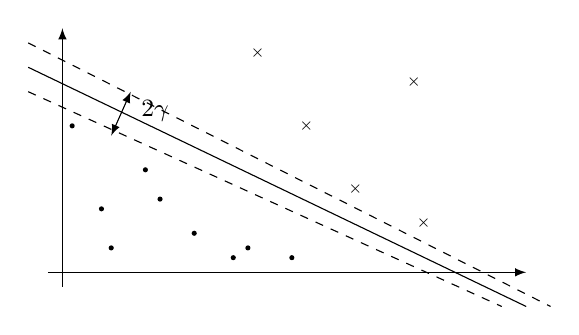
\begin{tikzpicture}[scale=0.62]
        \draw[->] (-.3,0) -- (9.5,0);
        \draw[->] (0,-.3) -- (0,5);
        \draw[-]    (-0.7,4.2) -- (9.5,-0.7);
        \draw[dashed] (-0.7,4.7) -- (10,-0.7);
        \draw[dashed] (-0.7,3.7) -- (9,-0.7);
        \draw[<->] (1,2.8) -- (1.4,3.7);
        \node at (1.9,3.3) {\small $2\gamma$};
        \foreach \px/\py in {5/3, 4/4.5, 6/1.7, 7.2/3.9, 7.4/1}{
          \node at (\px,\py) {\tiny $\times$};
        }
        \foreach \px/\py in {1/0.5, 0.8/1.3, 2/1.5, 3.8/0.5, 3.5/0.3, 0.2/3,
                             1.7/2.1, 4.7/0.3, 2.7/0.8}{
          \fill (\px,\py) circle (1.5pt);
        }
      \end{tikzpicture}
    \column{0.40\textwidth}
      \begin{itemize}
        \item Solid dots: class $-1$.
        \item Crosses: class $+1$.
        \item Dashed lines: margin boundaries.
        \item Points on dashed lines: \alert{support vectors}.
        \item All other points: irrelevant to the solution.
      \end{itemize}
  \end{columns}
\end{frame}

% ==========================================================================
\section{VC Dimension and Margin}
% ==========================================================================

\begin{frame}{VC Dimension of Linear Classifiers}
  \framesubtitle{Connecting margin to learnability}
  \begin{itemize}
    \item Unrestricted linear classifiers in $\mathbb{R}^d$: $\mathrm{VCdim} = d+1$.
    \item High $d$ $\Rightarrow$ large VC dimension $\Rightarrow$ potential overfitting.
    \item Yet SVMs often generalise well in very high (even infinite) dimensions.
    \item \alert{Resolution}: the margin constrains the effective capacity.
  \end{itemize}
  \vspace{0.5em}
  \begin{block}{Margin-based VC bound}
    If all data lie in a ball of radius $R$, the VC dimension of margin-$\gamma$ classifiers satisfies:
    \[
      \mathrm{VCdim} \;\lesssim\; \left(\frac{R}{\gamma}\right)^2.
    \]
    This bound is \alert{independent of the ambient dimension $d$}.
  \end{block}
\end{frame}

\begin{frame}{Margin as Regularisation}
  \framesubtitle{Why maximising margin prevents overfitting}
  \begin{itemize}
    \item Large margin $\Rightarrow$ small $(R/\gamma)^2$ $\Rightarrow$ small effective VC dimension.
    \item Smaller VC dimension $\Rightarrow$ tighter generalisation bounds.
    \item Generalisation bound schematically:
          \[
            \text{test error} \;\le\; \text{training error} + f\!\left(\frac{\mathrm{VCdim}}{n}\right).
          \]
    \item \alert{Maximising $\gamma$} reduces the complexity term without increasing training error.
  \end{itemize}
  \begin{block}{Key insight}
    Minimising $\|\w\|^2 \;\Leftrightarrow\; $ maximising margin $\;\Leftrightarrow\;$
    minimising an upper bound on the VC dimension.
    This is implicit regularisation.
  \end{block}
\end{frame}

% ==========================================================================
\section{Duality and the Dual SVM}
% ==========================================================================

\begin{frame}{Convex Duality: Overview}
  \framesubtitle{An alternative but equivalent view of the same problem}
  \begin{block}{Primal problem}
    \[
      \min_{\x\in\Omega} f(\x) \quad \text{s.t.}\quad g_i(\x) \le 0, \; i=1,\ldots,k.
    \]
  \end{block}
  \begin{itemize}
    \item Introduce \alert{Lagrange multipliers} $\lambda_i \ge 0$.
    \item \alert{Lagrangian}: $\mathcal{L}(\x,\Vlambda) = f(\x) + \sum_{i=1}^k \lambda_i g_i(\x)$.
    \item \alert{Dual function}: $D(\Vlambda) = \min_\x \mathcal{L}(\x,\Vlambda)$.
    \item Dual problem: $\max_{\Vlambda \succeq 0} D(\Vlambda)$.
  \end{itemize}
  \begin{alertblock}{Strong duality (Slater's condition)}
    When the primal is convex and strictly feasible, primal and dual optima coincide:
    $f^* = D^*$.
  \end{alertblock}
\end{frame}

\begin{frame}{KKT Conditions}
  \framesubtitle{Necessary and sufficient optimality conditions}
  At a primal-dual optimum $(\x^*, \Vlambda^*)$:
  \vspace{0.3em}
  \begin{enumerate}
    \item \textbf{Primal feasibility:} $g_i(\x^*) \le 0$.
    \item \textbf{Dual feasibility:} $\lambda_i^* \ge 0$.
    \item \textbf{Stationarity:} $\nabla_\x \mathcal{L}(\x^*,\Vlambda^*) = \mathbf{0}$.
    \item \textbf{Complementary slackness:} $\lambda_i^* g_i(\x^*) = 0$ for all $i$.
  \end{enumerate}
  \vspace{0.4em}
  \begin{itemize}
    \item Slackness: either the constraint is \alert{active} ($g_i=0$) or the multiplier is \alert{zero}.
    \item Inactive constraints do not contribute to the dual.
    \item This is the foundation of \alert{sparsity} in SVMs.
  \end{itemize}
\end{frame}

\begin{frame}{Hard-Margin SVM Lagrangian}
  \framesubtitle{Setting up the dual}
  \begin{itemize}
    \item Primal: $\min_{\w,b} \tfrac{1}{2}\|\w\|^2$ s.t.\ $t_i(\w^T\x_i+b)\ge 1$.
    \item Rewrite constraints as $g_i(\w,b) = 1 - t_i(\w^T\x_i+b) \le 0$.
  \end{itemize}
  \begin{block}{Lagrangian}
    \[
      \mathcal{L}(\w,b,\Vlambda) = \frac{1}{2}\|\w\|^2
      - \sum_{i=1}^n \lambda_i\bigl(t_i(\w^T\x_i+b) - 1\bigr).
    \]
  \end{block}
  Stationarity conditions ($\nabla_\w = \mathbf{0}$, $\partial/\partial b = 0$):
  \[
    \w^* = \sum_{i=1}^n \lambda_i t_i \x_i, \qquad
    \sum_{i=1}^n \lambda_i t_i = 0.
  \]
  \begin{itemize}
    \item \alert{Key insight}: $\w^*$ lies in the span of training examples (support vector expansion).
  \end{itemize}
\end{frame}

\begin{frame}{Hard-Margin Dual Problem}
  \framesubtitle{Maximise over multipliers only}
  Substituting $\w^*$ and the constraint into $\mathcal{L}$:
  \begin{block}{Dual SVM}
    \[
      \max_{\Vlambda} \;\left(\sum_{i=1}^n \lambda_i -
      \frac{1}{2}\sum_{i=1}^n\sum_{j=1}^n \lambda_i\lambda_j t_i t_j \x_i^T\x_j\right)
    \]
    \[
      \text{s.t.}\quad \lambda_i \ge 0, \quad \sum_{i=1}^n \lambda_i t_i = 0.
    \]
  \end{block}
  \begin{itemize}
    \item Primal: $d+1$ variables, $n$ constraints.
    \item Dual: $n$ variables, $1$ equality + nonnegativity constraints.
    \item Data appear only through \alert{inner products} $\x_i^T\x_j$ $\Rightarrow$ kernel trick applies.
  \end{itemize}
\end{frame}

\begin{frame}{Complementary Slackness and Support Vectors}
  \framesubtitle{Which points define the classifier?}
  KKT complementary slackness:
  \[
    \lambda_i^*\bigl(t_i(\w^{*T}\x_i + b^*) - 1\bigr) = 0.
  \]
  \begin{itemize}
    \item $\lambda_i^* > 0 \;\Rightarrow\; t_i(\w^{*T}\x_i+b^*) = 1$: point is on the margin $\Rightarrow$ \alert{support vector}.
    \item $\lambda_i^* = 0 \;\Rightarrow\;$ point is outside the margin; it does \alert{not} affect the solution.
  \end{itemize}
  \begin{block}{Sparse representation}
    \[
      \w^* = \sum_{i\in\mathcal{S}} \lambda_i^* t_i \x_i, \qquad
      \mathcal{S} = \{i \mid \lambda_i^* > 0\}.
    \]
    Only support vectors contribute. Typically $|\mathcal{S}| \ll n$.
  \end{block}
\end{frame}

\begin{frame}{Recovering the Bias and Prediction}
  \framesubtitle{From dual solution to classifier}
  \textbf{Bias $b^*$:} for any support vector $\x_k$ (active constraint $t_k(\w^{*T}\x_k+b^*)=1$):
  \[
    b^* = t_k - \sum_{j\in\mathcal{S}} \lambda_j^* t_j \x_j^T\x_k.
  \]
  Average over all support vectors for numerical stability.

  \vspace{0.5em}
  \textbf{Decision function:}
  \[
    y(\x) = \sum_{i\in\mathcal{S}} \lambda_i^* t_i \,\x_i^T\x + b^*.
  \]
  Predicted label: $\hat{t} = \mathrm{sign}(y(\x))$.
  \begin{itemize}
    \item Evaluation cost: proportional to $|\mathcal{S}|$, not $n$.
  \end{itemize}
\end{frame}

% ==========================================================================
\section{Soft-Margin SVM}
% ==========================================================================

\begin{frame}{Motivation: When Hard Margins Fail}
  \framesubtitle{Real data are rarely perfectly separable}
  \begin{itemize}
    \item Hard margin requires: $t_i(\w^T\boldsymbol{\phi}(\x_i)+b) \ge 1$ for \emph{all} $i$.
    \item If data are \alert{not linearly separable}: the system is infeasible.
    \item Even one mislabelled or noisy point can destroy the solution.
    \item We need a \alert{relaxation} that:
      \begin{itemize}
        \item tolerates some violations, and
        \item penalises them in a controlled way.
      \end{itemize}
  \end{itemize}
\end{frame}

\begin{frame}{Slack Variables}
  \framesubtitle{Measuring constraint violations}
  \begin{block}{Relaxed constraint}
    Introduce $\xi_i \ge 0$ for each training point:
    \[
      t_i(\w^T\boldsymbol{\phi}(\x_i)+b) \ge 1 - \xi_i.
    \]
  \end{block}
  \begin{center}
    \begin{tabular}{ll}
      \toprule
      Value of $\xi_i$ & Geometric meaning \\
      \midrule
      $0$ & Correctly classified, outside the margin \\
      $(0,1)$ & Correctly classified, \emph{inside} the margin \\
      $1$ & Exactly on the decision boundary \\
      $> 1$ & \alert{Misclassified} \\
      \bottomrule
    \end{tabular}
  \end{center}
  \begin{itemize}
    \item Slack variables provide a \alert{continuous} measure of violation.
    \item The problem remains feasible even when data overlap.
  \end{itemize}
\end{frame}

\begin{frame}{Soft-Margin Optimisation Problem}
  \framesubtitle{The $C$-SVM}
  \begin{block}{Primal (soft-margin SVM)}
    \[
      \min_{\w,b,\boldsymbol{\xi}} \;\frac{1}{2}\|\w\|^2 + C\sum_{i=1}^n \xi_i
    \]
    \[
      \text{s.t.}\quad t_i(\w^T\boldsymbol{\phi}(\x_i)+b) \ge 1-\xi_i,\quad \xi_i\ge 0.
    \]
  \end{block}
  \begin{itemize}
    \item $\tfrac{1}{2}\|\w\|^2$: \alert{margin maximisation} (as before).
    \item $C\sum_i \xi_i$: \alert{penalty} for violations.
    \item $C > 0$: regularisation parameter (selected by cross-validation).
      \begin{itemize}
        \item Large $C$: prioritise correct classification, smaller margin.
        \item Small $C$: larger margin, more violations allowed.
      \end{itemize}
  \end{itemize}
\end{frame}

\begin{frame}{Soft-Margin KKT Conditions}
  \framesubtitle{Stationarity and complementary slackness}
  Multipliers $\lambda_i \ge 0$ (margin constraints) and $\alpha_i \ge 0$ (slack $\ge 0$).

  Stationarity yields:
  \[
    \w^* = \sum_{i=1}^n \lambda_i t_i \boldsymbol{\phi}(\x_i), \quad
    \sum_{i=1}^n \lambda_i t_i = 0, \quad
    C - \lambda_i - \alpha_i = 0.
  \]
  Last equation $\Rightarrow \lambda_i \le C$ (since $\alpha_i \ge 0$).

  \vspace{0.4em}
  \begin{block}{Classification of training points}
    \begin{itemize}
      \item $\lambda_i^* = 0$: point outside margin, $\xi_i^* = 0$, not a support vector.
      \item $0 < \lambda_i^* < C$: on the margin boundary, $\xi_i^* = 0$ — \alert{classical support vector}.
      \item $\lambda_i^* = C$: inside margin or misclassified, $\xi_i^* > 0$ — \alert{margin-violating support vector}.
    \end{itemize}
  \end{block}
\end{frame}

\begin{frame}{Soft-Margin Dual Problem}
  \framesubtitle{The only change: upper bound on multipliers}
  \begin{block}{Dual (soft-margin SVM)}
    \[
      \max_{\Vlambda} \;\left(\sum_{i=1}^n \lambda_i -
      \frac{1}{2}\sum_{i,j} \lambda_i\lambda_j t_i t_j \kappa(\x_i,\x_j)\right)
    \]
    \[
      \text{s.t.}\quad \textcolor{TvAlert}{\mathbf{0 \le \lambda_i \le C}}, \quad
      \sum_{i=1}^n \lambda_i t_i = 0.
    \]
  \end{block}
  \begin{itemize}
    \item Identical to hard-margin dual, except $\lambda_i$ is now \textbf{bounded above by $C$}.
    \item As $C \to \infty$: reduces to the hard-margin dual.
    \item Data still appear only through \alert{kernel evaluations} $\kappa(\x_i,\x_j)$.
    \item Prediction: $y(\x) = \sum_{i\in\mathcal{S}} \lambda_i^* t_i \kappa(\x_i,\x) + b^*$.
  \end{itemize}
\end{frame}

% ==========================================================================
\section{SVM as Regularised Risk Minimisation}
% ==========================================================================

\begin{frame}{From Constraints to Unconstrained Objective}
  \framesubtitle{Eliminating slack variables analytically}
  For fixed $(\w,b)$, each $\xi_i$ is minimised independently:
  \[
    \xi_i^* = \max\!\bigl\{0,\; 1 - t_i(\w^T\boldsymbol{\phi}(\x_i)+b)\bigr\}.
  \]
  Substituting into the primal objective:
  \begin{block}{Unconstrained SVM objective}
    \[
      J(\w,b) = \frac{1}{2}\|\w\|^2 + C\sum_{i=1}^n
      \max\!\bigl\{0,\; 1 - t_i(\w^T\boldsymbol{\phi}(\x_i)+b)\bigr\}.
    \]
  \end{block}
  \begin{itemize}
    \item No constraints, no slack variables.
    \item Opens the door to \alert{gradient-based optimisation}.
  \end{itemize}
\end{frame}

\begin{frame}{Hinge Loss}
  \framesubtitle{The loss function underlying SVMs}
  \begin{block}{Definition}
    \[
      \ell_H(z_i) = \max\{0,\; 1 - t_i z_i\}, \quad z_i = \w^T\boldsymbol{\phi}(\x_i)+b.
    \]
  \end{block}
  \begin{itemize}
    \item Zero for correctly classified points \emph{outside} the margin.
    \item Positive (linear) penalty for points inside or on the wrong side.
  \end{itemize}
  \begin{block}{Regularised risk minimisation}
    \[
      J(\w,b) = \underbrace{\frac{1}{2}\|\w\|^2}_{\text{regulariser}}
      + \; C \underbrace{\sum_{i=1}^n \ell_H(z_i)}_{\text{empirical loss}}.
    \]
  \end{block}
  \begin{itemize}
    \item $C$ large: fits data more tightly.
    \item $C$ small: wider margin, stronger regularisation.
  \end{itemize}
\end{frame}

\begin{frame}{Subgradients of the Hinge Loss}
  \framesubtitle{Handling the non-differentiable kink}
  The hinge loss is \alert{not differentiable} at $t_i z_i = 1$.
  Use a \alert{subgradient} instead:
  \[
    \frac{\partial \ell_H}{\partial \w} =
    \begin{cases}
      \mathbf{0} & \text{if } t_i(\w^T\boldsymbol{\phi}(\x_i)+b) \ge 1, \\
      -t_i \boldsymbol{\phi}(\x_i) & \text{otherwise.}
    \end{cases}
  \]
  Subgradient of the full objective:
  \[
    \frac{\partial J}{\partial \w} = \w - C\sum_{i \in V} t_i \boldsymbol{\phi}(\x_i),
  \]
  where $V = \{i \mid t_i(\w^T\boldsymbol{\phi}(\x_i)+b) < 1\}$ is the set of \alert{violating points}.
  \begin{itemize}
    \item Only margin-violating examples drive the update.
    \item Correctly classified points with margin $\ge 1$: no contribution.
  \end{itemize}
\end{frame}

\begin{frame}{Gradient Descent Updates}
  \framesubtitle{Training SVMs with first-order methods}
  \begin{block}{Batch gradient descent step}
    \[
      \w^{(t+1)} = (1-\eta)\,\w^{(t)} + \eta C \sum_{i\in V^{(t)}} t_i\boldsymbol{\phi}(\x_i).
    \]
  \end{block}
  \begin{itemize}
    \item Factor $(1-\eta)$: \alert{weight decay} — implements regularisation.
    \item Additive term: corrects \alert{margin violations}.
    \item Variants: stochastic (SGD) and mini-batch — replace full sum by sample.
  \end{itemize}
  \begin{block}{Computational comparison}
    \begin{itemize}
      \item Dual QP solver: $O(n^3)$; accurate, sparse, kernel-ready.
      \item (S)GD on primal: $O(n)$ per epoch; scalable to large $n$.
    \end{itemize}
  \end{block}
\end{frame}

% ==========================================================================
\section{Extensions: Multiclass and Regression}
% ==========================================================================

\begin{frame}{Multiclass SVM: One-vs-All (OvA)}
  \framesubtitle{Reducing $K$-class to binary problems}
  \begin{block}{Strategy}
    Train $K$ binary SVMs. For class $k$: label $+1$ for class $k$, $-1$ for all others.
  \end{block}
  \begin{itemize}
    \item Each classifier gives a score:
          \[
            y_k(\x) = \sum_{i\in\mathcal{S}_k} \lambda_{i,k}^* t_{i,k} \kappa(\x_i,\x) + b_k^*.
          \]
    \item Prediction: $\hat{t} = \arg\max_{k} y_k(\x)$.
    \item Requires only $K$ training runs.
  \end{itemize}
  \begin{alertblock}{Caveat}
    Induced binary problems may be \alert{imbalanced} if $n_k \ll n$.
    Classifiers trained independently may give inconsistent scores.
  \end{alertblock}
\end{frame}

\begin{frame}{Multiclass SVM: One-vs-One (OvO)}
  \framesubtitle{Pairwise classifiers and majority voting}
  \begin{block}{Strategy}
    Train one binary SVM for \emph{every pair} of classes.
    \[
      \binom{K}{2} = \frac{K(K-1)}{2} \text{ classifiers.}
    \]
  \end{block}
  \begin{itemize}
    \item Each pairwise classifier is trained only on its two classes: less imbalance.
    \item Prediction: \alert{majority voting} — the class receiving most pairwise wins.
    \item Computational cost: $O(K^2)$ training runs.
  \end{itemize}
  \vspace{0.3em}
  \begin{center}
    \begin{tabular}{lcc}
      \toprule
      & OvA & OvO \\
      \midrule
      Number of SVMs & $K$ & $K(K-1)/2$ \\
      Training set per SVM & All $n$ & Class-pair subset \\
      Imbalance risk & High & Lower \\
      \bottomrule
    \end{tabular}
  \end{center}
\end{frame}

\begin{frame}{Support Vector Regression (SVR)}
  \framesubtitle{Extending SVMs to continuous outputs}
  \begin{itemize}
    \item Goal: predict a real value $y_i \in \mathbb{R}$ instead of a label.
    \item Central idea: introduce an \alert{$\epsilon$-insensitive tube} around the prediction.
  \end{itemize}
  \begin{block}{$\epsilon$-insensitive loss}
    \[
      L_\epsilon(y_i, \hat{y}_i) =
      \begin{cases}
        0 & |y_i - \hat{y}_i| \le \epsilon, \\
        |y_i - \hat{y}_i| - \epsilon & \text{otherwise.}
      \end{cases}
    \]
  \end{block}
  \begin{itemize}
    \item Points \emph{inside} the tube: zero loss $\Rightarrow$ they are \alert{not} support vectors.
    \item Points \emph{outside}: penalised linearly, they become support vectors.
    \item Encourages sparsity and robustness to small noise.
  \end{itemize}
\end{frame}

\begin{frame}{SVR: Primal Problem}
  \framesubtitle{Two sets of slack variables}
  Introduce $\xi_i \ge 0$ (upper violations) and $\xi_i^* \ge 0$ (lower violations):
  \begin{block}{SVR primal}
    \[
      \min_{\w,b,\boldsymbol{\xi},\boldsymbol{\xi}^*} \;\frac{1}{2}\|\w\|^2 +
      C\sum_{i=1}^n (\xi_i + \xi_i^*)
    \]
    \[
      \text{s.t.}\; y_i - \w^T\boldsymbol{\phi}(\x_i) - b \le \epsilon + \xi_i,\quad
      \w^T\boldsymbol{\phi}(\x_i)+b - y_i \le \epsilon + \xi_i^*.
    \]
  \end{block}
  \begin{itemize}
    \item Same trade-off as soft-margin SVM: $\|\w\|^2$ vs.\ violations.
    \item $\epsilon$: tube width; $C$: penalises out-of-tube deviations.
    \item Dual and prediction proceed exactly as in the classification case.
  \end{itemize}
\end{frame}

\begin{frame}{Computational Issues}
  \framesubtitle{Scaling SVMs to large datasets}
  \begin{alertblock}{Standard SVM training cost}
    Solving the dual QP: $O(n^3)$ — \alert{prohibitive} for large $n$.
  \end{alertblock}
  \vspace{0.4em}
  \begin{itemize}
    \item Research directions to speed up SVMs:
      \begin{itemize}
        \item \alert{Approximate QP solvers} (SMO, LIBSVM, etc.).
        \item \alert{Stochastic/mini-batch gradient descent} on the primal.
        \item Decomposition methods that work on subsets of variables.
      \end{itemize}
    \item Modern practice:
      \begin{itemize}
        \item Large $n$: gradient-based methods preferred.
        \item Moderate $n$, kernel required: dual QP solvers.
      \end{itemize}
  \end{itemize}
\end{frame}

% ==========================================================================
\section{Kernel Methods}
% ==========================================================================

\begin{frame}{Why Kernels?}
  \framesubtitle{Nonlinearity without explicit feature construction}
  \begin{itemize}
    \item Linear models: efficient, convex, analysable — but limited expressiveness.
    \item Naive fix: manually add polynomial or interaction features.
      \begin{itemize}
        \item Expensive to compute; feature dimension explodes.
        \item Requires domain expertise to choose which features.
      \end{itemize}
    \item \alert{Kernel trick}: behave \emph{as if} we worked in a rich feature space,
          but without constructing it explicitly.
  \end{itemize}
  \begin{block}{Core idea}
    Keep the algorithm \alert{linear in feature space}, making the decision boundary
    \alert{nonlinear in input space}, by replacing inner products with kernel evaluations.
  \end{block}
\end{frame}

\begin{frame}{Feature Maps and Kernel Functions}
  \framesubtitle{Formal setup}
  \begin{block}{Feature map}
    $\boldsymbol{\phi}: \mathcal{X} \to \mathcal{F}$ maps inputs to a (possibly infinite-dimensional)
    Hilbert space $\mathcal{F}$.
  \end{block}
  \begin{block}{Kernel function}
    \[
      \kappa(\x_i, \x_j) = \boldsymbol{\phi}(\x_i)^T \boldsymbol{\phi}(\x_j).
    \]
    Computes the inner product in $\mathcal{F}$ using only the original vectors.
  \end{block}
  \begin{itemize}
    \item SVM dual uses data only through $\x_i^T\x_j$.
    \item Replace with $\kappa(\x_i,\x_j)$: all computations remain in $\mathcal{X}$.
    \item $\boldsymbol{\phi}(\x)$ \alert{never needs to be formed explicitly}.
  \end{itemize}
\end{frame}

\begin{frame}{Valid Kernels: Mercer's Condition}
  \framesubtitle{When does a function define a valid inner product?}
  \begin{block}{Definition (positive semidefinite kernel)}
    $\kappa: \mathcal{X}\times\mathcal{X}\to\mathbb{R}$ is a valid kernel iff for every
    finite set $\{\x_1,\ldots,\x_n\}$ the \alert{Gram matrix}
    $K_{ij} = \kappa(\x_i,\x_j)$ is positive semidefinite:
    \[
      \mathbf{v}^T \mathbf{K}\,\mathbf{v} \ge 0 \quad\forall\,\mathbf{v}\in\mathbb{R}^n.
    \]
  \end{block}
  \begin{itemize}
    \item Guarantees existence of a Hilbert space $\mathcal{F}$ and feature map $\boldsymbol{\phi}$.
    \item Ensures SVM dual remains \alert{well-posed and convex}.
    \item Necessary and sufficient condition (Mercer's theorem).
  \end{itemize}
\end{frame}

\begin{frame}{Constructing Valid Kernels}
  \framesubtitle{Closure properties}
  If $\kappa_1, \kappa_2$ are valid kernels, then so are:
  \vspace{0.3em}
  \begin{columns}
    \column{0.48\textwidth}
      \begin{itemize}
        \item \textbf{Sum:} $\kappa_1 + \kappa_2$
        \item \textbf{Product:} $\kappa_1 \cdot \kappa_2$
        \item \textbf{Scalar multiple:} $c\,\kappa_1$, $c>0$
        \item \textbf{Exponential:} $e^{\kappa_1}$
      \end{itemize}
    \column{0.48\textwidth}
      \begin{itemize}
        \item \textbf{Polynomial:} $p(\kappa_1)$, $p$ with non-neg.\ coeffs
        \item \textbf{Weighted inner product:} $\x_1^T\mathbf{A}\x_2$, $\mathbf{A}\succ 0$
        \item \textbf{Scaling:} $f(\x_1)\kappa_1 g(\x_2)$
        \item \textbf{Composition:} $\kappa_3(\boldsymbol{\phi}(\x_1),\boldsymbol{\phi}(\x_2))$
      \end{itemize}
  \end{columns}
  \vspace{0.4em}
  \begin{itemize}
    \item \alert{Flexible kernel design}: combine simpler kernels into complex ones while
          preserving validity.
  \end{itemize}
\end{frame}

\begin{frame}{Polynomial Kernel}
  \framesubtitle{Controlled nonlinearity via degree}
  \begin{block}{Definition}
    \[
      \kappa(\x_1,\x_2) = (\x_1^T\x_2 + c)^d.
    \]
  \end{block}
  \begin{itemize}
    \item $d$: degree (complexity); $c$: balance between low- and high-order terms.
    \item Corresponds to a feature map with all monomials up to degree $d$.
    \item Example ($d=2$, $\mathbb{R}^2$): feature map
          $\boldsymbol{\phi}(\x) = (x_1^2,\,x_2^2,\,\sqrt{2}x_1x_2,\,\sqrt{2c}x_1,\,\sqrt{2c}x_2,\,c)^T \in \mathbb{R}^6$.
  \end{itemize}
  \begin{block}{Computational advantage}
    Evaluating $\kappa(\x_1,\x_2)$: $O(d)$ operations.\\
    Explicit degree-$d$ feature vector: $O(d^t)$ components.
    \alert{Exponential savings} via the kernel trick.
  \end{block}
\end{frame}

\begin{frame}{Gaussian (RBF) Kernel}
  \framesubtitle{Infinite-dimensional feature space}
  \begin{block}{Definition}
    \[
      \kappa(\x_1,\x_2) = \exp\!\left(-\frac{\|\x_1-\x_2\|^2}{2\sigma^2}\right).
    \]
  \end{block}
  \begin{itemize}
    \item Corresponds to an \alert{infinite-dimensional} feature map.
    \item Inner products computed exactly by the simple formula above.
    \item Validity: decompose as $e^{-\|\x_1\|^2/2\sigma^2} \cdot e^{\x_1^T\x_2/\sigma^2}
          \cdot e^{-\|\x_2\|^2/2\sigma^2}$ (product and scaling of valid kernels).
  \end{itemize}
  \begin{block}{Bandwidth $\sigma$ controls locality}
    \begin{itemize}
      \item Small $\sigma$: very local similarity, flexible/complex boundary, risk of \alert{overfitting}.
      \item Large $\sigma$: global/smooth similarity, risk of \alert{underfitting}.
      \item Tune by cross-validation.
    \end{itemize}
  \end{block}
\end{frame}

\begin{frame}{Common Kernels and When to Use Them}
  \framesubtitle{Choosing the right inductive bias}
  \begin{center}
    \renewcommand{\arraystretch}{1.3}
    \begin{tabular}{lll}
      \toprule
      Kernel & Formula & When to use \\
      \midrule
      Linear & $\x_1^T\x_2$ & Data approximately linearly separable \\
      Polynomial & $(\x_1^T\x_2+c)^d$ & Feature interactions matter \\
      Gaussian (RBF) & $\exp(-\gamma\|\x_1-\x_2\|^2)$ & Complex nonlinear structure \\
      Sigmoid & $\tanh(c_1\x_1^T\x_2+c_2)$ & Neural-net analogy (use with care) \\
      \bottomrule
    \end{tabular}
  \end{center}
  \begin{itemize}
    \item Gaussian is the \alert{default choice} when no prior knowledge is available.
    \item Performance of Gaussian degrades in very high dimensions (distance concentration).
    \item Sigmoid kernel is \alert{not always valid} — check conditions.
  \end{itemize}
\end{frame}

\begin{frame}{Kernelised SVM: The Full Picture}
  \framesubtitle{Combining duality, sparsity, and kernels}
  \begin{block}{Kernelised soft-margin dual}
    \[
      \max_{\Vlambda} \;\left(\sum_{i=1}^n \lambda_i -
      \frac{1}{2}\sum_{i,j}\lambda_i\lambda_j t_i t_j \kappa(\x_i,\x_j)\right)
    \]
    \[
      \text{s.t.}\quad 0\le\lambda_i\le C,\quad \sum_i\lambda_i t_i = 0.
    \]
  \end{block}
  \begin{block}{Prediction}
    \[
      y(\x) = \sum_{i\in\mathcal{S}} \lambda_i^* t_i \kappa(\x_i,\x) + b^*.
    \]
  \end{block}
  \begin{itemize}
    \item \alert{Nonlinearity} entirely in the kernel; algorithm is convex throughout.
    \item \alert{Sparsity} preserved: only support vectors matter.
    \item \alert{Kernel choice} = encoding domain knowledge about similarity.
  \end{itemize}
\end{frame}

% ==========================================================================
\section{Summary}
% ==========================================================================

\begin{frame}{Key Results at a Glance}
  \framesubtitle{Summary}
  \begin{center}
    \renewcommand{\arraystretch}{1.4}
    \footnotesize
    \begin{tabular}{ll}
      \toprule
      Result & Formula / Statement \\
      \midrule
      Hard-margin primal & $\min \tfrac{1}{2}\|\mathbf{w}\|^2$ s.t.\ $t_i(\mathbf{w}^T\mathbf{x}_i+b)\ge 1$ \\
      Hard-margin dual & $\max \sum\lambda_i - \tfrac{1}{2}\sum_{ij}\lambda_i\lambda_j t_it_j\mathbf{x}_i^T\mathbf{x}_j$ \\
      Soft-margin primal & $\min \tfrac{1}{2}\|\mathbf{w}\|^2 + C\sum\xi_i$ s.t.\ relaxed constraints \\
      Soft-margin dual & Same as hard, but $0\le\lambda_i\le C$ \\
      Geometric margin & $\gamma = 1/\|\mathbf{w}\|$ (after normalisation) \\
      VC bound (margin) & $\mathrm{VCdim}\lesssim(R/\gamma)^2$ \\
      Hinge loss & $\ell_H = \max\{0, 1-t_i z_i\}$ \\
      Kernel trick & Replace $\mathbf{x}_i^T\mathbf{x}_j$ with $\kappa(\mathbf{x}_i,\mathbf{x}_j)$ \\
      Gaussian kernel & $\exp(-\|\mathbf{x}_1-\mathbf{x}_2\|^2/2\sigma^2)$ \\
      Polynomial kernel & $(\mathbf{x}_1^T\mathbf{x}_2+c)^d$ \\
      \bottomrule
    \end{tabular}
  \end{center}
\end{frame}

%\begin{frame}{The Big Picture}
%  \framesubtitle{Where do SVMs fit?}
%  \begin{center}
%  \begin{tikzpicture}[
%      node distance=1.2cm and 2.2cm,
%      box/.style={draw, rounded corners, fill=TvLight, minimum width=2.8cm, minimum height=0.7cm,
%                  align=center, font=\small},
%      alertbox/.style={draw, rounded corners, fill=TvAlert!20, minimum width=2.8cm,
%                        minimum height=0.7cm, align=center, font=\small},
%      arr/.style={->, thick, color=TvMid}
%    ]
%    \node[box] (linear) {Linear classifier\\in $\mathcal{F}$};
%    \node[box, right=of linear] (margin) {Maximise\\margin};
%    \node[box, right=of margin] (dual) {Dual formulation\\(QP)};
%    \node[box, below=of dual] (sparse) {Sparse solution\\(support vectors)};
%    \node[box, below=of margin] (kernel) {Kernel trick\\$\kappa(\mathbf{x}_i,\mathbf{x}_j)$};
%    \node[alertbox, below=of linear] (nonlin) {Nonlinear decision\\boundary in $\mathcal{X}$};
%
%    \draw[arr] (linear) -- (margin);
%    \draw[arr] (margin) -- (dual);
%    \draw[arr] (dual) -- (sparse);
%    \draw[arr] (dual) -- (kernel);
%    \draw[arr] (kernel) -- (nonlin);
%    \draw[arr] (sparse) -- (nonlin);
%  \end{tikzpicture}
%  \end{center}
%\end{frame}

%\end{document}
